%Install required packages (AMS-LaTeX, natbib, textcase, and bm)

\documentclass[aps,pra,reprint,superscriptaddress]{revtex4-1}
\usepackage{graphicx}
\usepackage{fullpage}
\usepackage{upgreek}
\usepackage{verbatim}
\usepackage{graphicx,epstopdf}
\usepackage{xcolor}
\usepackage{braket}
%\usepackage{gensymb}

\bibliographystyle{apsrev4-1}

\begin{document}


\title{Imaging small numbers of Ba atoms in solid xenon for barium tagging in nEXO} 

%putting \newline in next to J Albert makes the linew break, but then makes us start at left, uncentered ...
%\author{\hspace{30mm} T.~Walton}
\author{T.~Walton}
\affiliation{Physics Department, Colorado State University, Fort Collins CO, USA}
\author{C.~Chambers}
\affiliation{Physics Department, Colorado State University, Fort Collins CO, USA}
\author{A.~Craycraft}
\affiliation{Physics Department, Colorado State University, Fort Collins CO, USA}
\author{W.~Fairbank Jr.}\thanks{Corresponding author}
\affiliation{Physics Department, Colorado State University, Fort Collins CO, USA}
%\author{\newline \newline J.B.~Albert}
%\author{\newline J.B.~Albert}
\author{J.B.~Albert}
\affiliation{Physics~Department~and~CEEM,~Indiana~University,~Bloomington~IN,~USA}
\author{D.J.~Auty}
\affiliation{Department of Physics and Astronomy, University of Alabama, Tuscaloosa AL, USA}
\author{P.S.~Barbeau}
\affiliation{Department of Physics, Duke University, and Triangle Universities Nuclear Laboratory (TUNL), Durham North Carolina, USA}
\author{ V. ~Basque}
\affiliation{Physics Department, Carleton University, Ottawa ON, Canada}
\author{D.~Beck}
\affiliation{Physics Department, University of Illinois, Urbana-Champaign IL, USA}
\author{M.~Breidenbach}
\affiliation{SLAC National Accelerator Laboratory, Stanford CA, USA}
\author{T.~Brunner}
\affiliation{Physics Department, Stanford University, Stanford CA, USA}
\affiliation{Department of Physics, McGill University, Montreal QC, Canada}
\author{G.F.~Cao}
\affiliation{Institute of High Energy Physics, Beijing, China}
\author{B.~Cleveland}\thanks{Also SNOLAB, Sudbury ON, Canada}
\affiliation{Department of Physics, Laurentian University, Sudbury ON, Canada}
\author{M.~Coon}
\affiliation{Physics Department, University of Illinois, Urbana-Champaign IL, USA}
\author{T.~Daniels}
\affiliation{SLAC National Accelerator Laboratory, Stanford CA, USA}
\author{S.J.~Daugherty}
\affiliation{Physics~Department~and~CEEM,~Indiana~University,~Bloomington~IN,~USA}
\author{R.~DeVoe}
\affiliation{Physics Department, Stanford University, Stanford CA, USA}
\author{T.~Didberidze}
\affiliation{Department of Physics and Astronomy, University of Alabama, Tuscaloosa AL, USA}
\author{J.~Dilling}
\affiliation{TRIUMF, Vancouver BC, Canada}
\author{M.J.~Dolinski}
\affiliation{Department of Physics, Drexel University, Philadelphia PA, USA}
\author{M.~Dunford}
\affiliation{Physics Department, Carleton University, Ottawa ON, Canada}
\author{L.~Fabris}
\affiliation{Oak Ridge National Laboratory, Oak Ridge TN, USA}
\author{J.~Farine}
\affiliation{Department of Physics, Laurentian University, Sudbury ON, Canada}
\author{W.~Feldmeier}
\affiliation{Technische Universitat Munchen, Physikdepartment and Excellence Cluster Universe, Garching, Germany}
\author{P.~Fierlinger}
\affiliation{Technische Universitat Munchen, Physikdepartment and Excellence Cluster Universe, Garching, Germany}
\author{D.~Fudenberg}
\affiliation{Physics Department, Stanford University, Stanford CA, USA}
\author{G.~Giroux}\thanks{Now at Queen's University, Kingston ON, Canada}
\affiliation{LHEP, Albert Einstein Center, University of Bern, Bern, Switzerland}
\author{R.~Gornea}
\affiliation{Physics Department, Carleton University, Ottawa ON, Canada}
\affiliation{LHEP, Albert Einstein Center, University of Bern, Bern, Switzerland}
\author{K.~Graham}
\affiliation{Physics Department, Carleton University, Ottawa ON, Canada}
\author{G.~Gratta}
\affiliation{Physics Department, Stanford University, Stanford CA, USA}
\author{M.~Heffner}
\affiliation{Lawrence Livermore National Laboratory, Livermore CA, USA}
\author{M.~Hughes}
\affiliation{Department of Physics and Astronomy, University of Alabama, Tuscaloosa AL, USA}
\author{X.S.~Jiang}
\affiliation{Institute of High Energy Physics, Beijing, China}
\author{T.N.~Johnson}
\affiliation{Physics~Department~and~CEEM,~Indiana~University,~Bloomington~IN,~USA}
\author{S.~Johnston}
\affiliation{Amherst Center for Fundamental Interactions and Physics Department, University of Massachusetts, Amherst MA, USA}
\author{A.~Karelin}
\affiliation{Institute for Theoretical and Experimental Physics, Moscow, Russia}
\author{L.J.~Kaufman}
\affiliation{Physics~Department~and~CEEM,~Indiana~University,~Bloomington~IN,~USA}
\author{R.~Killick}
\affiliation{Physics Department, Carleton University, Ottawa ON, Canada}
\author{T.~Koffas}
\affiliation{Physics Department, Carleton University, Ottawa ON, Canada}
\author{S.~Kravitz}
\affiliation{Physics Department, Stanford University, Stanford CA, USA}
\author{R.~Kr\"ucken}
\affiliation{TRIUMF, Vancouver BC, Canada}
\author{A.~Kuchenkov}
\affiliation{Institute for Theoretical and Experimental Physics, Moscow, Russia}
\author{K.S.~Kumar}
\affiliation{Department of Physics and Astronomy, Stony Brook University, SUNY, Stony Brook NY,USA}
\author{\color{red}D.S.~Leonard}
\affiliation{\color{red}New place in S. Korea}
\author{C.~Licciardi}
\affiliation{Physics Department, Carleton University, Ottawa ON, Canada}
\author{Y.H.~Lin}
\affiliation{Department of Physics, Drexel University, Philadelphia PA, USA}
\author{J.~Ling}
\affiliation{Physics Department, University of Illinois, Urbana-Champaign IL, USA}
\author{R.~MacLellan}
\affiliation{Department of Physics, University of South Dakota, Vermillion SD, USA}
\author{M.G.~Marino}
\affiliation{Technische Universitat Munchen, Physikdepartment and Excellence Cluster Universe, Garching, Germany}
\author{B.~Mong}
\affiliation{Department of Physics, Laurentian University, Sudbury ON, Canada}
\author{D.~Moore}
\affiliation{Physics Department, Stanford University, Stanford CA, USA}
\author{A.~Odian}
\affiliation{SLAC National Accelerator Laboratory, Stanford CA, USA}
\author{I.~Ostrovskiy}
\affiliation{Physics Department, Stanford University, Stanford CA, USA}
\author{A.~Piepke}
\affiliation{Department of Physics and Astronomy, University of Alabama, Tuscaloosa AL, USA}
\author{A.~Pocar}
\affiliation{Amherst Center for Fundamental Interactions and Physics Department, University of Massachusetts, Amherst MA, USA}
\author{F.~Retiere}
\affiliation{TRIUMF, Vancouver BC, Canada}
\author{P.C.~Rowson}
\affiliation{SLAC National Accelerator Laboratory, Stanford CA, USA}
\author{M.P.~Rozo}
\affiliation{Physics Department, Carleton University, Ottawa ON, Canada}
\author{A.~Schubert}
\affiliation{Physics Department, Stanford University, Stanford CA, USA}
\author{D.~Sinclair}
\affiliation{TRIUMF, Vancouver BC, Canada}
\affiliation{Physics Department, Carleton University, Ottawa ON, Canada}
\author{E.~Smith}
\affiliation{Department of Physics, Drexel University, Philadelphia PA, USA}
\author{V.~Stekhanov}
\affiliation{Institute for Theoretical and Experimental Physics, Moscow, Russia}
\author{M.~Tarka}
\affiliation{Department of Physics and Astronomy, Stony Brook University, SUNY, Stony Brook NY,USA}
\author{T.~Tolba}
\affiliation{LHEP, Albert Einstein Center, University of Bern, Bern, Switzerland}
\author{K.~Twelker}\thanks{Now at WiTricity, Watertown, MA}
\affiliation{Physics Department, Stanford University, Stanford CA, USA}
\author{J.-L.~Vuilleumier}
\affiliation{LHEP, Albert Einstein Center, University of Bern, Bern, Switzerland}
\author{J.~Walton}
\affiliation{Physics Department, University of Illinois, Urbana-Champaign IL, USA}
\author{M.~Weber}
\affiliation{Physics Department, Stanford University, Stanford CA, USA}
\author{L.J.~Wen}
\affiliation{Institute of High Energy Physics, Beijing, China}
\author{U.~Wichoski}
\affiliation{Department of Physics, Laurentian University, Sudbury ON, Canada}
\author{L.~Yang}
\affiliation{Physics Department, University of Illinois, Urbana-Champaign IL, USA}
\author{Y.-R.~Yen}
\affiliation{Department of Physics, Drexel University, Philadelphia PA, USA}
\author{Y.B.~Zhao}
\affiliation{Institute of High Energy Physics, Beijing, China}

\collaboration{nEXO Collaboration}

\date{\today}

\begin{abstract}
Images of Ba atoms in solid Xe in a focused laser region, after deposition from vacuum onto a cold sapphire window, are obtained using a 619-nm fluorescence peak down to the single-atom level.  This is an important step toward barium tagging with a cryogenic probe from liquid Xe for the nEXO neutrinoless double beta decay experiment.

\end{abstract}

\pacs {32.30.-r,32.50.+d,32.90.+a,14.60.Pq,23.40.-s} % insert suggested PACS numbers in braces on next line

\maketitle %\maketitle must follow title, authors, abstract and \pacs

\section{Introduction}

The search for neutrinoless double beta decay ($0\nu\beta\beta$) is an important probe into the nature of neutrinos.  Observation would require that neutrinos are Majorana particles, would demonstrate violation of lepton number conservation, and could help determine the absolute neutrino mass \cite{ReviewNuMass}.  EXO-200 is searching for $0\nu\beta\beta$ in \textsuperscript{136}Xe with around 170~kg of liquid Xe (lXe) enriched to 80.6\% \textsuperscript{136}Xe in a dual time projection chamber (TPC).  Two-neutrino double beta decay ($2\nu\beta\beta$) of \textsuperscript{136}Xe has been observed by EXO-200, and its half-life is measured at $T^{2\nu\beta\beta}_{1/2} = 2.165 \pm 0.016$(stat)$ \pm 0.059$(sys)$ \times 10^{21}$~yr \cite{EXO200TwoNuLong}.  The most recent EXO-200 $0\nu\beta\beta$ search sets a limit on the half-life at $T^{0\nu\beta\beta}_{1/2} < 1.1 \times 10^{25}$~yr (90\% CL), which corresponds to an effective Majorana neutrino mass of $\braket{m_{\nu_{e}}} < $190-450~meV, depending on nuclear matrix element calculations \cite{EXO200ZeroNuNature}. % nEXO, the ton-scale successor to EXO-200, will search for $0\nu\beta\beta$ with a much larger mass of enriched \textsuperscript{136}Xe.

A lXe TPC has a unique opportunity to tag the daughter at the site of a double beta decay event, which would improve $0\nu\beta\beta$ sensitivity by effectively eliminating all backgrounds \cite{Moe1991}.  Ba tagging is being investigated for possible incorporation in the next-generation ton-scale lXe experiment, nEXO.  A few techniques for Ba tagging are under investigation \cite{Twelker2014}{\color{gray}[hot probe paper?]}, including one for a possible future Xe gas TPC \cite{Brunner2015}.  The method described here is for barium tagging in the nEXO lXe TPC, in which a cryogenic probe would be moved to the position of the $0\nu\beta\beta$ candidate in order to freeze the daughter ion into a small amount of solid Xe (sXe) at the end of the probe.  It would then be detected by its laser-induced fluorescence in the sXe.

The spectroscopy of Ba in sXe is described in the previous work \cite{Mong2015}.  An image of $\leq 10^4$ Ba atoms was obtained with the strong fluorescence peaks at 577 and 591 nm.  However, bleaching of these fluorescence peaks with laser exposure reduces the emission at these wavelengths rapidly at high laser intensity, e.g., using a focused beam.  Thus obtaining large numbers of photons from single Ba atoms is difficult without a method to overcome bleaching, e.g., with repumping lasers.  Imaging was not attempted in \cite{Mong2015} with the peak at 619~nm, though this peak has weaker bleaching by many orders of magnitude.  This peak is promising for more sensitive imaging of smaller numbers of atoms because larger numbers of photons per atom may be obtained.

It is expected that a Ba\textsuperscript{++} ion will neutralize once to Ba\textsuperscript{+} in lXe, as the lXe conduction band gap is slightly less than the ionization potential for Ba\textsuperscript{+} \cite{Moe1991}.  It is also not known whether the Ba\textsuperscript{++} might neutralize completely in the charge cloud following a $\beta\beta$ event.  A new study of neutralization of alpha decay daughters in the EXO-200 lXe TPC is in the process of publication [ref? arxiv? example of arxiv ref in 2014 nu review, [185]].  As a result, the feasibility of detecting single Ba ions as well as atoms is still of interest.  This work focuses on imaging single Ba atoms in sXe via the low-bleaching 619-nm fluorescence.  Varying numbers of atoms are observed in a focused laser region down to the single atom level\emph{\color{gray}, and images of separate single atoms on a single deposit are obtained by scanning the focused laser}.

\section{Apparatus and Method}

The apparatus for depositing and observing Ba/Ba\textsuperscript{+} deposits in sXe is described in \cite{Mong2015}.  Important components are shown in Fig. \ref{fig:apparatus}.  The source of Ba\textsuperscript{+} is an ion beam at 2000~eV, filtered to select Ba\textsuperscript{+} with an E$\times$B velocity filter.  A set of pulsing plates produces 1-$\mu$s pulses for depositing small numbers of ions.  The spectra of Ba\textsuperscript{+} ion deposits in the sXe matrix exhibit peaks known to be due to neutral Ba atoms \cite{Mong2015}.  Thus some percentage of the ions neutralize in the matrix, but the fraction has not yet been determined.  An alternative source of neutral Ba is a BaAl$_{4}$ getter wire which can be inserted to emit Ba atoms toward the sample.  However, it is challenging to achieve low Ba flux with this source and to calibrate it.

\begin{figure}
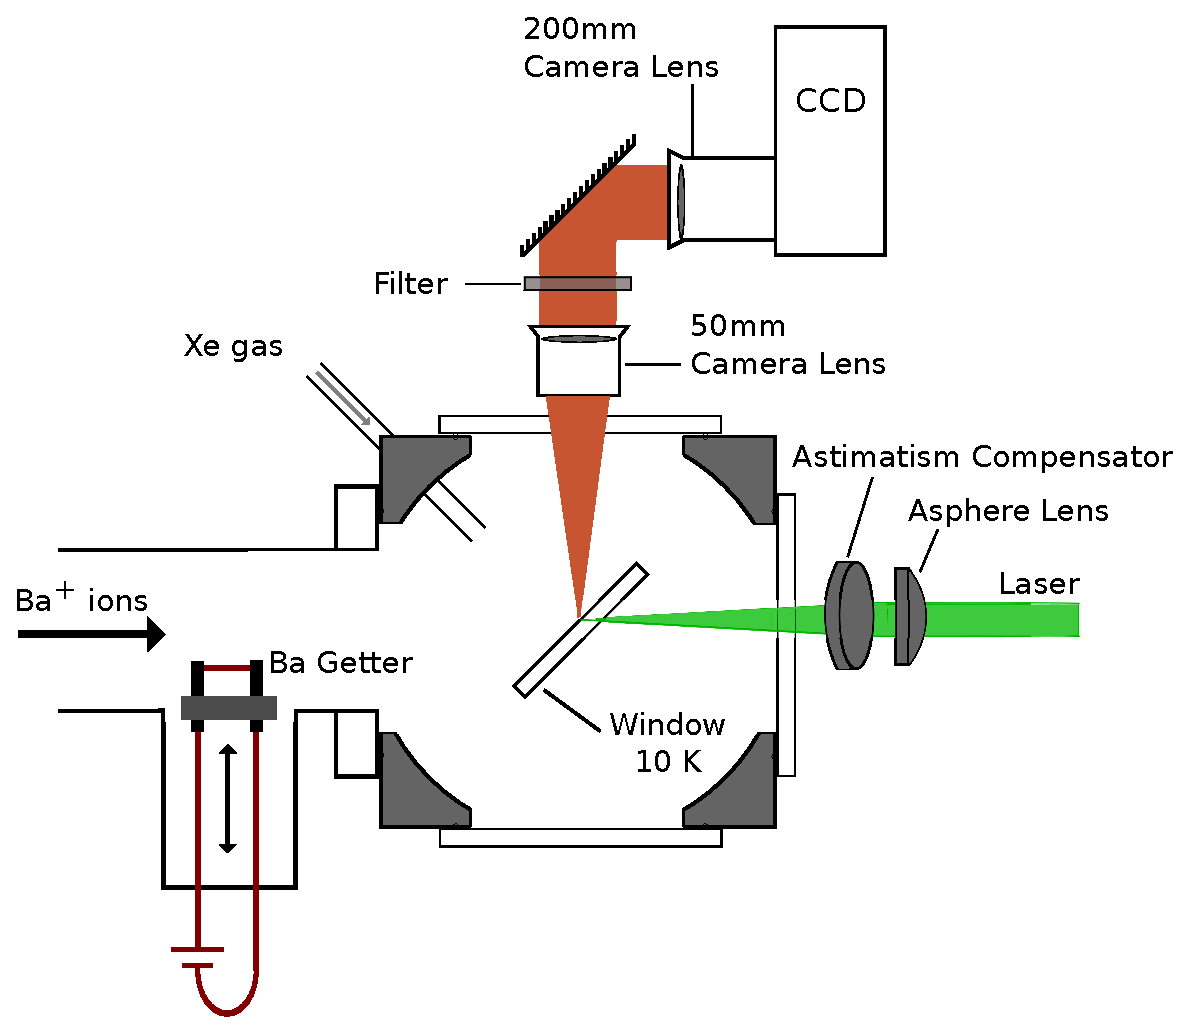
\includegraphics[width=0.5\textwidth]{figures/cryo_inkscape_chris_full.eps}
\caption{Experimental setup for depositing Ba/Ba\textsuperscript{+} in sXe matrices, and for excitation and observation.  {\color{gray}\emph{want to put compensator in, and depict laser lens as asphere.}}}
\label{fig:apparatus}
\end{figure}

Deposits are made on a cold sapphire window tilted at 45$^{\circ}$.  To create a sample, Xe gas is directed toward the window using a leak valve. The Xe gas freezes on the window and forms a sXe matrix with a thickness of a few hundred nanometers.  This is initiated a few seconds prior to the Ba deposit, continues during the Ba deposit, and is turned off a few seconds after the Ba deposit.

In this work, deposits are made with the sapphire window at around 50~K, partly to reduce hydrogen content in the matrix, as hydrogen freezes well below 50~K in vacuum \cite{Mong2015}.  The window is then cooled to 11~K for observation.  Deposits made at 50~K result in higher 619-nm signal than those made at 11~K, likely due to a higher population of 619-nm matrix sites.  Xe deposition at around 30~nm/s also results in higher 619-nm signal, as compared to lower leak rates, while not being so high as to result in a frosty Xe matrix.  An experiment cycle consists of a deposit at 50 K and a fluorescence observation at 11 K;  then the deposit is evaporated by heating the window to 100 K.  Many deposits are made in a day with varying numbers of ions deposited, as well as periodic Xe-only deposits to establish the background.

The excitation laser, a Coherent 599 cw dye laser with Rhodamine 6G dye pumped by the 514-nm line of a Lexel 3500 argon ion laser, enters from the back side of the window.  Ba fluorescence light is collected and collimated by a 50~mm Nikon camera lens.  A band-pass filter with FWHM of 20~nm passes just the 619-nm fluorescence peak.  A 200~mm Nikon camera lens then focuses the image onto a liquid nitrogen cooled CCD, resulting in an image of 4x magnification.  Each of the 20$\times$20 $\mu$m pixels of the CCD represents approximately 5$\times$5 $\mu$m on the SXe sample.

For a given laser intensity, the smallest focus possible is desired for optimal signal-to-noise from single atoms.  To achieve this, an aspherical lens of 7.9~cm focal length is used to minimize spherical aberration, and a fused silica optical flat of 1~cm thickness is placed at 10$^{\circ}$ after the lens in order to compensate for astigmatism caused by the tilted sapphire window (see Fig. \ref{fig:apparatus}).

%end of Bill's comments on 1e

\section{Results}
\label{sec:results}

%{\color{gray}[The excitation spectrum for the 619-nm peak is shown in Fig. \ref{fig:excitspec}.  An excitation wavelength of 570~nm is used.]}

%\begin{figure}
%\includegraphics[width=0.48\textwidth]{figures/excitspec.png}
%\caption{Excitation spectrum for the 619-nm emission peak.  The discontinuity is due to use of different laser dyes, Rhodamine 110 and Rhodamine 6G.  The vertical scale is fluorescence normalized to laser power with an arbitrary scaling.}
%\label{fig:excitspec}
%\end{figure}

A typical image made with a focused laser beam at 570~nm is shown in Fig. \ref{fig:image_example}.  The laser's path through the sapphire window is seen as a weak vertical line.  At both ends, some background emission from the surfaces is observed.  At the front surface (at the top in the image), extra fluorescence is detected from a small number of Ba atoms within the focused laser.

\begin{figure}
\includegraphics[width=0.4\textwidth]{figures/raw_14-atom_labels.png}
\caption{Example image of Ba\textsuperscript{+} deposit in focused laser.  Pixels are $5~\mu$m$ \times 5~\mu$m.}
\label{fig:image_example}
\end{figure}

The number of Ba\textsuperscript{+} ions deposited within the 1/e radius of the laser beam gives a rough upper limit to the number of Ba atoms responsible for the observed signal.  For ion pulses of 13~fC/pulse and a focused laser 1/e\textsuperscript{2} radius of w$_{0}$ = 2.1~$\mu$m \emph{\color{gray}I get 2.06~$\mu$m for x and 2.66~$\mu$m for y, 2.36~$\mu$m average}, this results in about 0.05 Ba\textsuperscript{+} ions/pulse in the above area.  The signal in Fig. \ref{fig:image_example} corresponds to a deposit of about 14 Ba\textsuperscript{+} ions into the laser region, and is therefore roughly due to $\leq$ 14 Ba atoms.  A $\leq$ 56-atom deposit (56 ions deposited) is shown in Fig. \ref{fig:XeBaXe}b, with Xe-only deposits made before and after (Fig. \ref{fig:XeBaXe}a,c)).  It is important that no Ba is left over after evaporating the sample, even for larger deposits.

\begin{figure}
\includegraphics[width=0.5\textwidth]{figures/Xe-Ba-Xe_56-atom_71-73-74.png}
\caption{Image of a 56-ion deposit with local sXe-only deposits: (a) sXe-only, (b) $\leq$ 56 atoms in sXe, (c) sXe-only.  Pixels are $5~\mu$m$ \times 5~\mu$m.}
\label{fig:XeBaXe}
\end{figure}

\begin{figure}
\includegraphics[width=0.48\textwidth]{figures/lin_20150807_postXe.png}
\caption{619-nm Ba fluorescence vs. number of ions deposited.  {\color{blue}\emph{Could use better ion beam consistency.}}}
\label{fig:ctsVsIons}
\end{figure}

The counts vs. ions deposited are plotted in Fig. \ref{fig:ctsVsIons}.  Observe the linearity in summed CCD counts, from the image of the laser region in the sXe, vs. ions deposited for several deposits.  Each point has subtracted the counts from a nearby Xe-only run.  The observed signal corresponds to about 2000~counts/mW per atom with 60-s CCD exposures.  Counts are scaled by laser power to account for small variations in laser power.

To obtain images of Ba fluorescence, sXe-only images are subtracted {\color{gray}[This isn't said in explanation of linearity plot because those do not directly subtract images, they subtract integrated counts after using integration regions specific to each run (due to slight movements)]}.  A subtracted image of a deposit corresponding to a single Ba atom is shown in Fig. \ref{fig:lego}.  A solitary peak is observed from the Ba in the laser region.

%\begin{figure}[h!tb]
%	\includegraphics[width=0.45\textwidth]{figures/lego_varying.png}
%	\includegraphics[width=0.45\textwidth]{figures/lego_statistical.png}
%	\caption{Images of small numbers of Ba atoms in a focused laser beam.  {\color{red}Maybe need to specify conditions.}}
%	\label{fig:lego}
%\end{figure}

\begin{figure}
\includegraphics[width=0.48\textwidth]{figures/lego_near-line_1-atom.png}
\caption{Image of a single Ba atom (on average) in a focused w = 2.1~$\mu$m laser beam, with 60~s exposure of 0.18~mW laser power.}
\label{fig:lego}
\end{figure}

A Gaussian fit to the images gives a 1/e$^{2}$ radius of about 12~$\mu$m, which is much larger than the laser beam radius of w = 2.1~$\mu$m.  Aberrations and vibrations in the collection optics and imperfections in the surface of the sXe layer could contribute to blurring of the image.  Relative motion of the laser and the window could also lead to image broadening and to exposure of more Ba atoms than calculated above.  The latter effect has been checked by observing images of the focused laser relative to a reference point on the sapphire window on time frames down to 50~ms.  Vibrations were observed on the order of 15~$\mu$m in x and 4~$\mu$m in y, mainly due to cryostat vibrations, which corresponds to a total coverage of about {\color{red}7} times the laser region.  However, the signal at a given time still comes from an area the size of the laser region.  Thus, the signals observed correspond to an average number of atoms according to the laser spot size, though the total number of atoms responsible is about {\color{red}7} times larger.
%The latter effect has been checked by measuring intensity variations of the laser beam and its reflection from the window when cut 50\% by a razor blade.  {\color{blue}Maximum vibrations observed were on the order of ?~$\mu$m and ?~$\mu$m peak-peak for the laser and reflection, respectively}.

\subsection{Scanned Images}

\emph{\color{blue}Put scanned image of single atoms here.}

\subsection{Identification of 619-nm Peak as Ba in sXe}

Deposits made with the neutral Ba getter source are compared to a Ba\textsuperscript{+} deposit in Fig. \ref{fig:ion_getter_ar}.  Identical spectra are observed using the different sources under similar deposit conditions, confirming the identification of neutral Ba.  Another peak at 670~nm which is mentioned in \cite{Mong2015} is also attributed to Ba, likely in another Xe matrix site.  Observing Ba in the 619-nm matrix site at the low-energy (thermal) deposit from the getter is also good news for the prospect of grabbing Ba/Ba\textsuperscript{+} on a probe out of lXe.

\begin{figure}
\includegraphics[width=0.48\textwidth]{figures/getter_ion_Ar_calibrated.png}
\caption{Observation of deposits from three different sources in sXe.  Curves are scaled due to different deposit sizes.}
\label{fig:ion_getter_ar}
\end{figure}

An absence of fluorescence is observed from deposits of Ar\textsuperscript{+} in sXe (Fig. \ref{fig:ion_getter_ar}).  Ar\textsuperscript{+} ions are deposited with the same ion beam, also at 2000~eV, and under the same conditions.  This further rules out any matrix-damage-related sources of the 619-nm peak, such as fluorescent color centers.

%Ion currents of 30~nA and Xe deposition rates of 50~nm/s result in a Xe:Ba ratio of around 10\textsuperscript{4}:1.  This is 10~x higher than the recommended host:guest ratio [ref that old paper ... well, Brian's thesis says itand it's probably in that book you have to buy] for isolating Ba atoms in the matrix.

%{\color{red}I'm having trouble re-producing this, so maybe we leave it out:  }{\color{gray}Finally, a measurement of the Ba\textsuperscript{+} beam velocity confirms a mass of $137(?) \pm ?$, ruling out any contribution of barium oxide }(But probably not BaHx\textsuperscript{+}){{\color{gray}in the beam.  This is possible by knowing (a) the energy of the ions (2000~eV), (b) the time between the signals in a set of induction plates and the Faraday cup as well as the distance between the two, and (c) the timing of those signals for a pulse of Ar\textsuperscript{+} at the same energy, whose mass we know.  }

%{\color{gray}[Is there a statement we can make about molecules with lighter (O2, N2, H2, ...) being likely to show us mode peaks?]}


%\subsection{Temperature Dependence}

%Bad:  The temperature dependence of the 619-nm fluorescence is shown in Fig. \ref{fig:anneal} through three annealing cycles of a deposit made at 11~K.  The first anneal results in an overall larger signal upon returning to 11~K.  In anneal 2, lower fluorescence is observed at higher temperature, but essentially no signal is lost after returning to 11~K.  Anneal 3, to higher temperature of 48~K, does result in loss of overall signal.  {\color{red}[\textbf{If this is confusing or not relevant to the paper, we should leave out the whole subsection of temp. dependence, but not much was said about the 619 peak in the spec. paper.  I meant for this to show the fact that we need to be this cold to observe the peak in vacuum}]}  This temperature dependence of the fluorescence means that the probe in nEXO may need to be moved to a location out of the lXe where it can be cooled to 10 - 15~K.

%\begin{figure}
%\includegraphics[width=0.5\textwidth]{figures/anneal_green_20140916_runs34-37_bg64_v12_618nm.png}
%\caption{Observing 619-nm peak through annealing process of a deposit made at 11~K.  {\color{red}[Will need nicer plot if we show this]}}
%\label{fig:anneal}
%\end{figure}

%\section{Discussion}

%It is worth noting that the initially lower amplitude of the 619-nm peak, vs. the peaks around 590~nm, does not imply anything about their relative populations.  Different matrix sites can have very different effects on electron transition rates, and fluorescence efficiencies can be quite different.  In fact, the fluorescence efficiency of the 619-nm site is measured to be {\color{red}$1 \times 10^{-5}$}, calculated using the cross section of Ba in sXe reported in \cite{Mong2015}.

\subsection{Backgrounds}
\label{sec:backgrounds}

Very low concentrations of Cr\textsuperscript{3+} in the sapphire bulk (sub-ppb level) produce a broad fluorescence, the tail of which enters the 610-630~nm region passed by the band-pass filter and produces the faintly visible line through the sapphire window discussed above.  This fluorescence is identified as Cr\textsuperscript{3+} by its excitation spectrum, identical to that of the well-known lines around 693~nm.  \emph{\color{gray}Show figure?}  Commercially available c-plane quality sapphire \emph{\color{gray}(mention Meller?)} has sufficiently low concentrations for the 619-nm single atom signal level.

Another background is observed on the surfaces of the window, also caused by laser excitation.  This is more of a nuisance, as it not as easily distinguished from the Ba in an image.  It also exhibits bleaching, which can cause confusion in subtractions, though its bleaching rate is different from that of the 619-nm Ba emission.  \emph{\color{gray}(Mention temp.-dependence?)}  To minimize this, the window is exposed to the laser until the background reaches a steady value.  The set of deposits used for Fig. \ref{fig:ctsVsIons} was done after about an hour of pre-exposure of the sapphire window to the focused laser.

%Note that backgrounds due to impurities are not expected in the high-purity lXe environment of nEXO.

%\emph{\color{gray}Do we want a bleaching section?}

\section{Conclusions}

The 619-nm emission peak observed in deposits of Ba\textsuperscript{+} and Ba in sXe is attributed to neutral Ba \emph{\color{gray}in a stable and relatively abundant matrix site}.
%An excitation spectrum and temperature dependence of the fluorescence are reported.
Images of 619-nm fluorescence in a focused laser region from Ba atoms are achieved down to an average number of Ba atoms at the single-atom level.  Successful detection of Ba atoms in sXe at this level is a significant step toward Ba tagging in nEXO. 

\section*{Acknowledgements}

Shon Cook and Brian Mong for pioneering work and primary authorship in \cite{Mong2015}.  This material is based upon work supported by the National Science Foundation under Grant Nunber PHY-1132428 and the U.S. Department of Energy, Office of Science, Office of High Energy Physics \textbf{\textcolor{red}{under Award Number DE-FG02-03ER41255.}}

%\bibliography{references10}
\begin{thebibliography}{00}
 \bibitem{ReviewNuMass} K.A. Olive \emph{et al.} (Particle Data Group), ``14. Neutrino Mass, Mixing, and Oscillations," \emph{Chin. Phys. C} \textbf{38}, 090001 (2014) (http://pdg.lbl.gov).

%\bibitem{anticorr} E. Conti \emph{et al.}, \emph{Phys. Rev. B} \textbf{68}, 054201 (2003).

\bibitem{EXO200TwoNuLong} J. Albert \emph{et al.} (EXO-200 Collaboration), \emph{Phys. Rev. C} \textbf{89}, 015502 (2014).

\bibitem{EXO200ZeroNuNature} J. Albert \emph{et al.} (EXO-200 Collaboration), \emph{Nature} \textbf{510}, 229 (2014).

\bibitem{Moe1991} M. Moe, Phys. Rev. C \textbf{44}, R931 (1991).

\bibitem{Twelker2014} K. Twelker \emph{ et al.}, Review of Scientific Instruments \textbf{85}, 095114 (2014).

\bibitem{Brunner2015} T. Brunner \emph{ et al.}, International Journal of Mass Spectrometry {\color{red}\textbf{379} (2015) 110-120.}

\bibitem{Mong2015} B. Mong \emph{ et al.}, Phys. Rev. A \textbf{91}, 022505 (1954).
\end{thebibliography}

\end{document}